\section{Adaptation in Chapel}\label{sec:adaptation_in_chapel}

%\section{Chapel Language Features Necessary for Modulo Unrolling}\label{sec:language_features}

The goal of this section is to present our adaptation in Chapel of the modulo unrolling WU optimization presented in Section \ref{sec:transformation}. We also provide a basic understanding of zippered iteration and array slicing, two important features in Chapel used in the optimization's implementation. 

\subsection{Chapel Zippered Iteration}\label{sec:zippered_iteration}

Iterators are a widely used language feature in the Chapel programming language. Chapel iterators are blocks of code that are similar to functions and methods except that iterators can return multiple values back to the call site with the use of the \textit{yield} keyword instead of \textit{return}. Iterators are commonly used in loops to traverse data structures in a particular fashion. For example, an iterator $fibonacci(n: int)$ might be responsible for yielding the first $n$ Fibonacci numbers. This iterator could then be called in a loop's header to execute iterations 0, 1, 1, 2, 3, and so on. Arrays themselves are iterable in Chapel by default. This is how Chapel can support other important language features such as scalar promotion and whole array assignment. 

Chapel allows multiple iterators of the same size and shape to be iterated through simultaneously. This is known as \textit{zippered iteration} \cite{chamberlain2011user}, and an example is shown in Figure \ref{affine_loop}b. When zippered iteration is used, corresponding iterations are processed together. On each loop iteration, an $n$-tuple is generated, where $n$ is the number of items in the zippering. The $d^{th}$ component of the tuple generated on loop iteration $j$ is the $j^{th}$ item that would be yielded by iterator $d$ in the zippering. 

Zippered iteration can be used with either sequential \textbf{for} loops or parallel \textbf{forall} loops in Chapel. Parallel zippered iteration is implemented in Chapel using leader-follower semantics. That is, a \textit{leader} iterator is responsible for creating tasks and dividing up the work to carry out the parallelism. A \textit{follower} iterator performs the work specified by the leader iterator for each task and generally resembles a serial iterator. 

\subsection{Chapel Array Slicing}\label{sec:array_slicing}

Chapel supports another useful language feature known as \textit{array slicing}. This feature allows portions of an array to be accessed and modified in a succinct fashion. For example, consider two arrays $A$ and $B$ containing indices from $1..10$. Suppose we wanted to assign elements $A[6]$, $A[7]$, and $A[8]$ to elements $B[1]$, $B[2]$, and $B[3]$ respectively. We could achieve this in one statement by writing $B[1..3] = A[6..8]$. Here, $A[6..8]$ is a slice of the original array $A$, and $B[1..3]$ is a slice of the original array $B$. 

In Chapel, an array slice can support a range of elements with a stride in some cases. For example, in the previous example, we could have made the assignment $B[1..3] = A[1..6$ $by$ $2]$. This would have assigned elements $A[1]$, $A[3]$, and $A[5]$ to elements $B[1]$, $B[2]$, and $B[3]$ respectively. Since all array slices in Chapel are arrays themselves, array slices are also iterable. 

\begin{figure}
	\begin{center}
	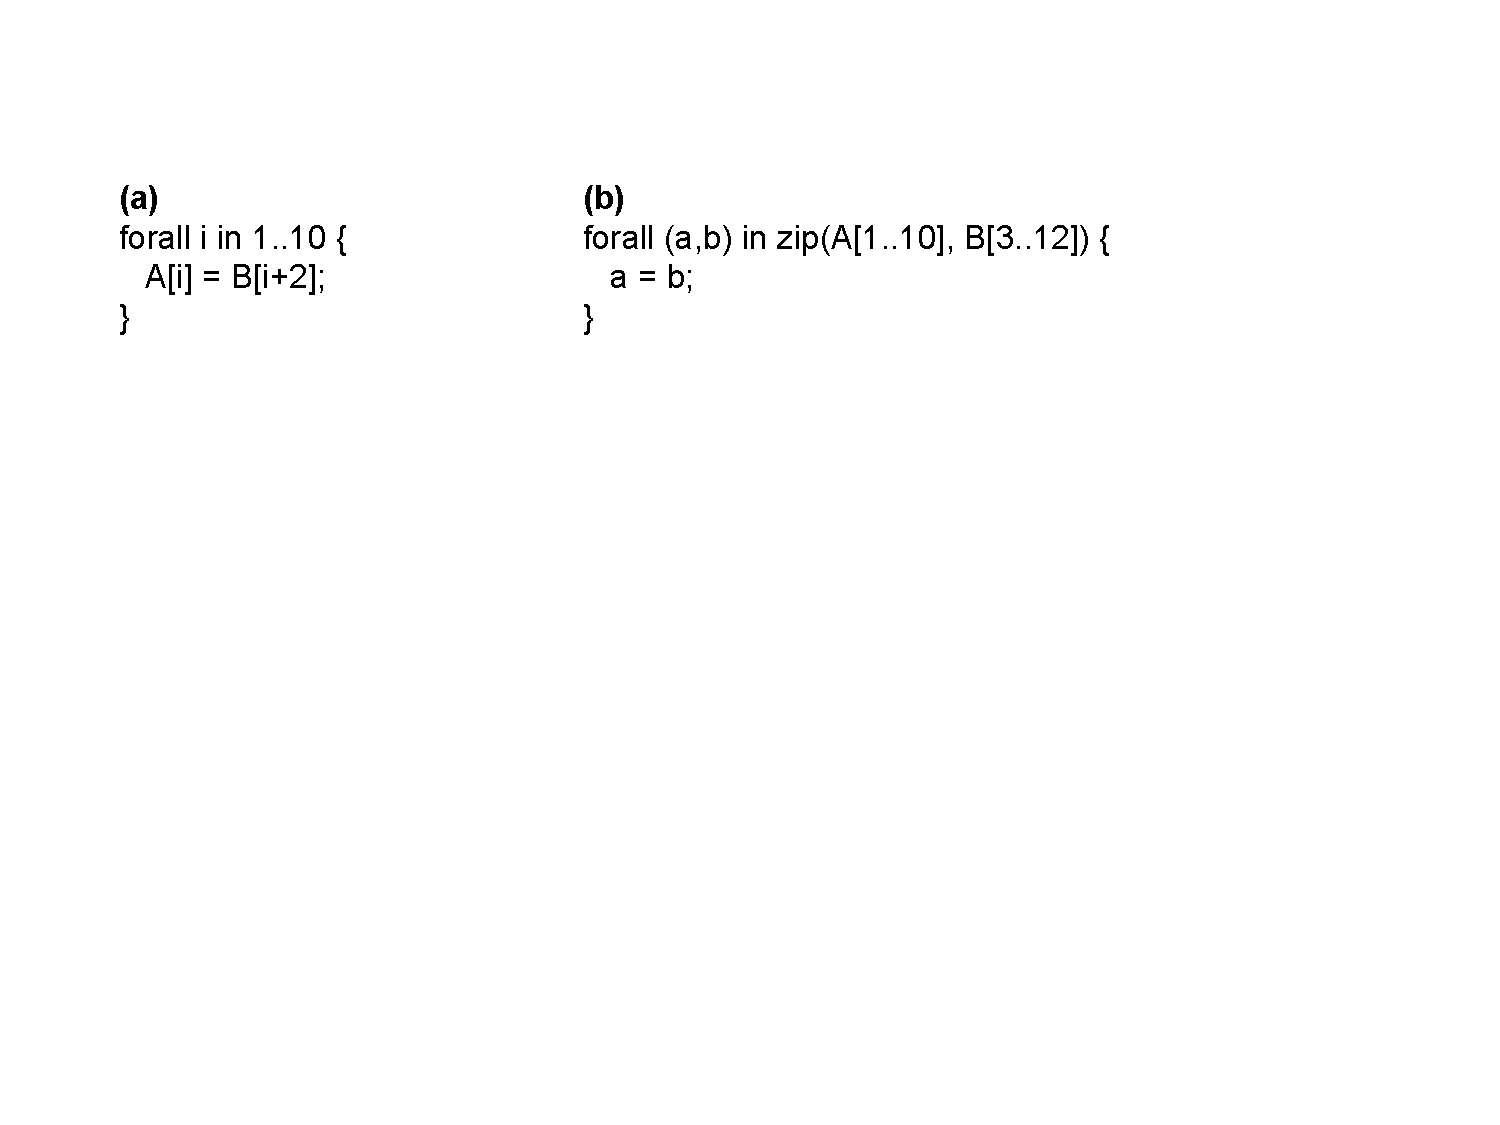
\includegraphics[scale=0.50]{./Figures/affine_loop}
	\caption{(a) Chapel loop written using a single loop induction variable $i$ ranging from 1 to 10. The loop contains two affine array accesses. (b) The same loop written using zippered iterators in Chapel. Instead of a loop induction variable and a range of values to denote the loop bounds, two array slices each containing the 10 elements accessed by the loop in (a) are specified.}
	\label{affine_loop}
	\end{center}
\end{figure}

Together, array slicing and parallel zippered iteration can express any parallel affine loop in Chapel that uses affine array accesses. Each affine array access in the loop body is replaced with a corresponding array slice in the loop header, which produces the same elements as the original loop. 

Consider the code fragment in Figure \ref{affine_loop}a. There are two affine array accesses $A[i]$ and $B[i+2]$ in Figure \ref{affine_loop}a. The loop is written in a standard way where the loop induction variable $i$ takes on values from 1 to 10. Because the loop is a \textbf{forall} loop, loop iterations are not guaranteed to complete in a specific order. This loop assigns elements of array $B$ to $A$ such that the $i^{th}$ element of $A$ is equal to the $(i+2)^{th}$ element of $B$ after the loop finishes. In Figure \ref{affine_loop}b, the same loop is written using zippered iterators. The loop induction variable $i$ no longer needs to be specified, and each affine array access has been replaced with an array slice in the zippering of the loop header. It is possible to transform an affine loop in this fashion even when an affine array access has a constant factor multiplied by the loop induction variable. The resulting array slice will contain a stride equal to the constant factor. The two loops in Figure \ref{affine_loop} are equivalent and generate the same results, but they differ in their execution.

Because any parallel affine loop can be transformed into an equivalent parallel loop that uses zippered iteration, we observe a natural place in the Chapel programming language in which to implement modulo unrolling WU: the leader and follower iterators of the Cyclic and Block Cyclic distribution. The leader iterator divides up the loop's iterations according to the locales they are executed on and passes this work to each follower iterator in the zippering. The follower iterator can then perform the aggregation of remote data elements according to the work that has been passed to it. 

\begin{comment}
\begin{figure}
	\begin{center}
	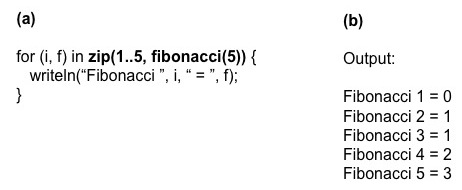
\includegraphics[scale=0.60]{./Figures/zippered_iteration}
	\caption{(a) Chapel code fragment showing a loop using zippered iteration. A tuple of loop index variables equal to the number of items in the zippering is declared in the loop header. If $j$ is the current loop iteration, variable $i$ is equal to the $j^{th}$ element in the range $1..5$, and $f$ corresponds to the $j^{th}$ element in the iterator $fibonacci(5)$. The \textit{zip} keyword tells the loop header which items to iterate over using zippered iteration. (b) Program output of the code fragment in Figure~\ref{zippered_iteration}a.}
	\label{zippered_iteration}
	\end{center}
\end{figure}
\end{comment}

\begin{figure}
	\begin{center}
	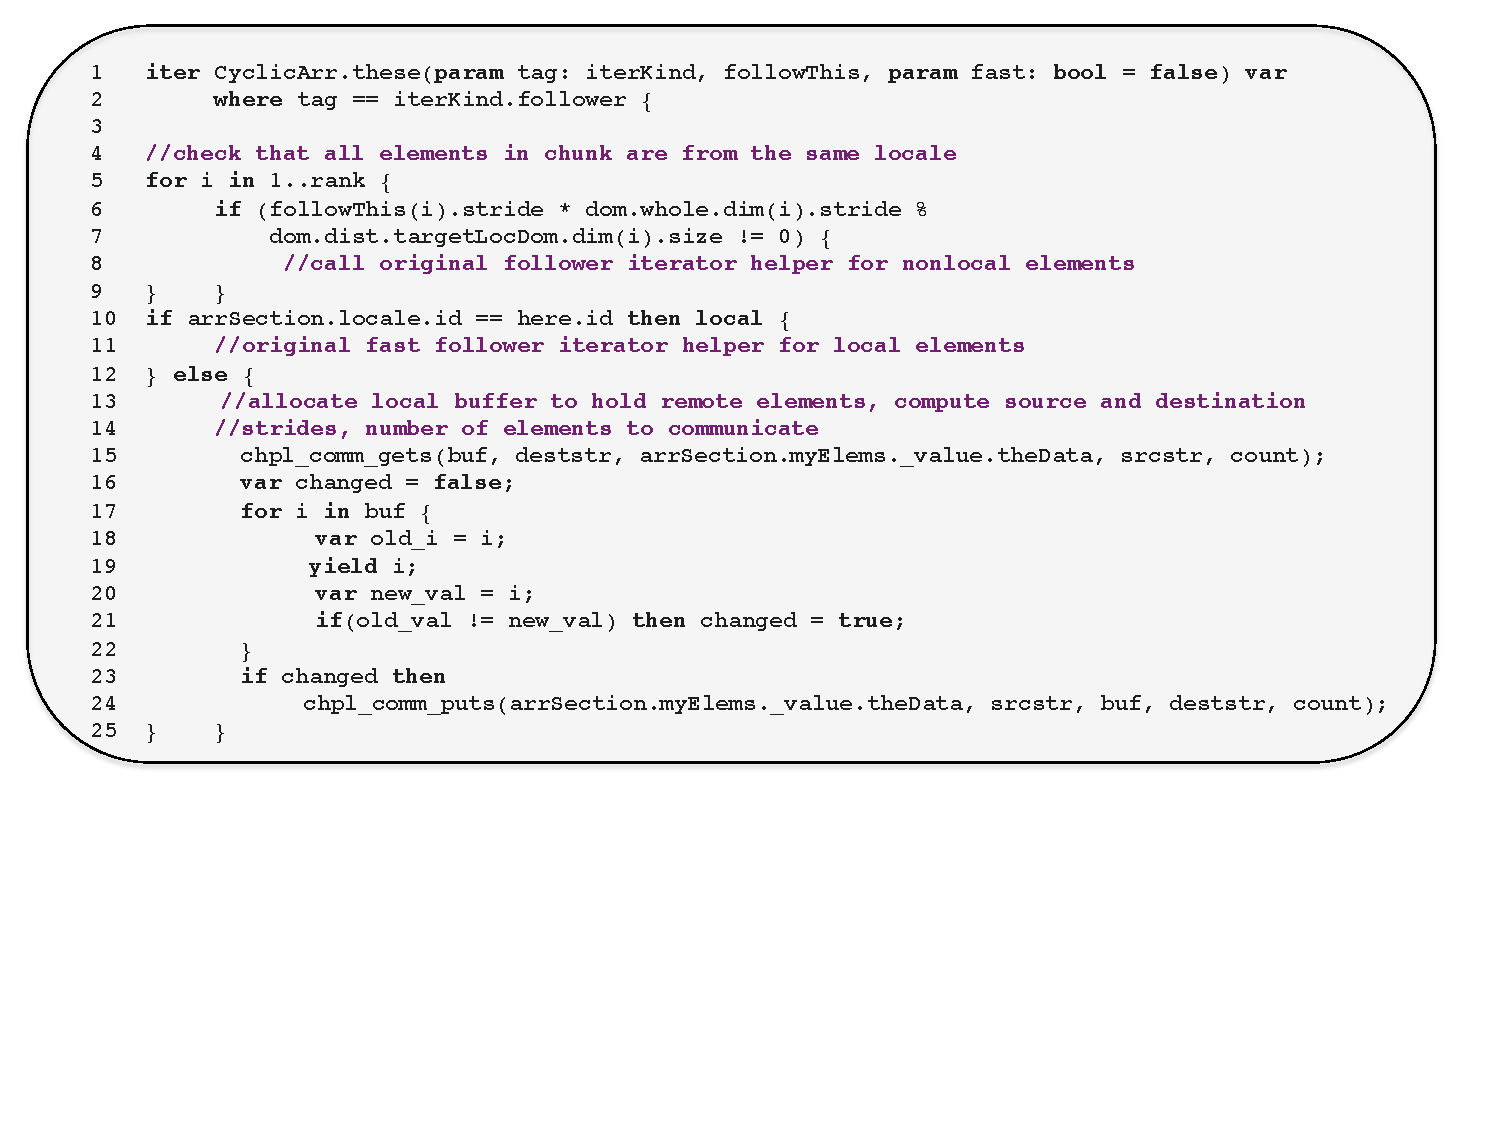
\includegraphics[scale=0.40]{./Figures/cyclic_muwu_follower}
	\caption{Cyclic with modulo unrolling WU caption}
	\label{cyclic_muwu_follower}
	\end{center}
\end{figure}

\subsection{Cyclic Distribution with Modulo Unrolling WU}\label{subsec:cyclic_modulo}

\begin{comment}
Modulo unrolling WU is implemented in the follower iterator of the Cyclic distribution. Based on the semantics of parallel zippered iteration, the leader iterator will divide up the iterations of the loop across the locales of the machine according to the first item in the zippering. This could mean that some portions of work will not be local to where the computation is taking place. The follower iterator in the Cyclic distribution recognizes whether or not its chunk of work is local or remote. If remote, all of the remote array elements are brought to the present locale in a local buffer using one \texttt{chpl\_comm\_gets} call. Finally, elements of the local buffer are now yielded back to the loop header. A loop body may modify the elements that are yielded to it via zippered iteration. To account for this, the follower iterator compares the element before it was yielded to the element after it was yielded. If any of the elements in the follower's chunk of work were modified, the entire local buffer is stored back to the remote local via one \texttt{chpl\_comm\_puts} call. 
\end{comment}

\subsection{Block Cyclic Distribution with Modulo Unrolling WU}\label{subsec:block_cyclic_modulo}

\begin{comment}
For the Chapel Block Cyclic implementation, both the leader and follower iterators have been modified to support the modulo unrolling WU optimization. Modulo unrolling, in its original form, is not compatible with the Block Cyclic distribution because consecutive array elements can reside on the same locale (this is defined by the block size parameter), which destroys the static locality information that we were able to use in the Cyclic distribution. The Block Cyclic leader iterator is now modified to choose slices of work such that the new "stride" is equal to the product of the block size and the cycle size. This way, when the work is passed to the follower iterator, elements that are in the same position within each block are guaranteed to be on the same locale. The follower iterator of the Block Cyclic distribution can now perform modulo unrolling WU in the same way as the Cyclic distribution. 
\end{comment}